\documentclass[12pt, french]{article}
\usepackage{tikz}
\usepackage{circuitikz}
\usepackage{pgfplots}
\pgfplotsset{compat=1.16}
\usepackage{fancyhdr, fancybox, lastpage}
\usepackage[most]{tcolorbox}
\usepackage[a4paper, margin={0.3in, .75in}]{geometry}
\usepackage{wrapfig}
\pagestyle{fancy}
\renewcommand\headrulewidth{1pt}
\renewcommand\footrulewidth{1pt}
\fancyhf{}
\rhead{ \em{Zakaria Haouzan}}
\lhead[C]{\em{2ème année baccalauréat Sciences Mathématiques}}
\chead[C]{}
\rfoot[C]{}
\lfoot[R]{}
\cfoot[]{\em{Page \thepage / \pageref{LastPage}}}


\newtcolorbox{Box2}[2][
enhanced,
breakable,
]{
                lower separated=false,
                colback=white,
colframe=white!20!black,fonttitle=\bfseries,
colbacktitle=white!30!gray,
coltitle=black,
enhanced,
attach boxed title to top left={yshift=-0.1in,xshift=0.15in},
title=#2,#1}


\begin{document}
\begin{center}
	\shadowbox {\bf{Dipôle RC }}
\end{center}

\vspace{-0.2cm}
%\begin{wrapfigure}{r}{0.22\textwidth}
%\begin{center}
%\vspace{-0.6cm}
%\includegraphics[width=0.22\textwidth]{./img/Ex2.png}
%\end{center}
%\end{wrapfigure}



%%_________________________Exercice ! :"_________________________Exercice
\begin{Box2}{Exercice 1 :Le condensateur réel}
	Dans un circuit ouvert comportant un condensateur chargé, se produit une décharge progressive et lente de ce condensateur au cours du temps. La durée de décharge dépend de la qualité du diélectrique du condensateur. Un tel condensateur est appelé condensateur réel ou condensateur imparfait et peut-être modélisé par une association en parallèle d'un condensateur parfait de capacité $C$ et d'un conducteur ohmique de résistance $R_d$ (Résistance de fuite) (figure 1).

	\begin{center}
		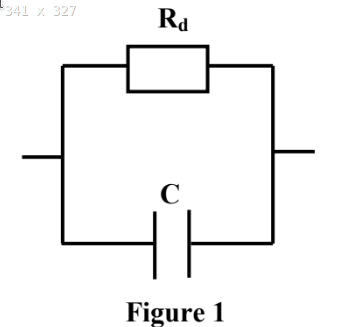
\includegraphics[width=0.16\textwidth]{./img/Ex00_C.png}
		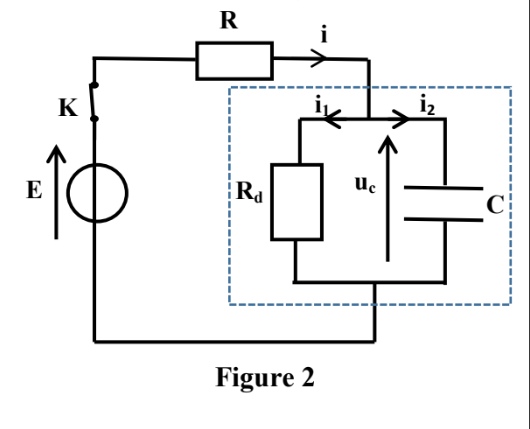
\includegraphics[width=0.27\textwidth]{./img/Ex00_C1.png}
		%\captiocc{}
	\end{center}




	\subsubsection*{1- Charge d'un condensateur réel}
	Le circuit électrique de la figure 2 comporte :

	\begin{itemize}
		\item Un générateur de tension de f.e.m. $E$
		\item Un conducteur ohmique de résistance $R$
		\item Un condensateur réel de capacité $C=5\mu F$ et de résistance de fuite $R_d$
		\item Un interrupteur $K$
	\end{itemize}

	A un instant pris comme origine des dates $t=0$, on ferme l'interrupteur $K$.

	1.1- Vérifier que l'expression de l'intensité $i$ du courant dans le circuit s'écrit:
	\[ i = \frac{1}{R_d}u_C + C\frac{du_C}{dt} \]

	1.2- Montrer que l'équation différentielle vérifiée par la tension $u_C$ entre les armatures du condensateur s'écrit :
	\[ \frac{du_C}{dt} + \frac{u_C}{\tau} = A \]
	avec $\tau = \frac{R.R_d.C}{R+R_d}$ et $A = \frac{E}{R.C}$

	\begin{wrapfigure}[5]{r}{0.33\textwidth}
		\begin{center}
			\vspace{-3cm}
			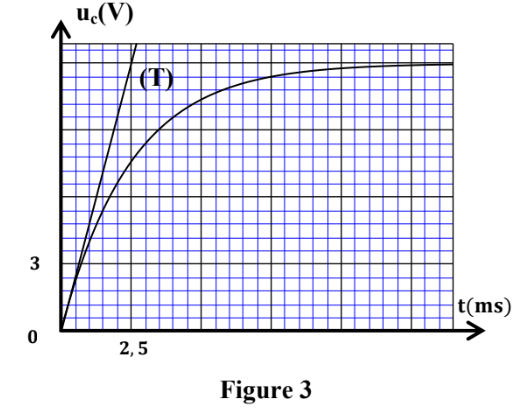
\includegraphics[width=0.33\textwidth]{./img/Ex00_Cr.png}
		\end{center}
	\end{wrapfigure}


	1.3- Déduire, au régime permanent, l'expression de la tension maximale $u_{C(max)}$ en fonction de $R_d$, $R$ et $E$. Comparer $u_{C(max)}$ à $E$.

	1.4- On considère que $R_d \gg R$. Un dispositif adéquat a permis de tracer l'évolution de la tension $u_C$ en fonction du temps $t$ (figure 3). ((T) représente la tangente à la courbe à l'instant $(t=0)$). En exploitant la courbe, déterminer la valeur de $E$ et celle de $R$.
	\subsubsection*{2-Décharge du condensateur réel dans le cas où $R_d \gg R$}
	Lorsque le régime permanent est établi, on ouvre l'interrupteur $K$ à un instant considéré comme une nouvelle origine des dates $t=0$.

	2.1- Établir l'équation différentielle vérifiée par la charge $q(t)$ du condensateur.

	2.2- La solution de l'équation différentielle est de la forme : $q(t)=\beta e^{-\lambda t}$ avec $\lambda$ et $\beta$ deux constantes positives.

	2.2.1- Sachant que la tension entre les armatures du condensateur prend la valeur $u_1=10V$ à la date $t_1=12min$. Trouver la valeur de $R_d$.

	2.2.2- Soit $p=\frac{\xi_J}{\xi_0}$ la proportion de l'énergie dissipée par effet joule dans le circuit, avec $\xi_0$ l'énergie électrique emmagasinée dans le condensateur à $t=0$ et $\xi_J$ l'énergie dissipée par effet joule dans la résistance de fuite $R_d$. Calculer $p$ à l'instant $t_1$.



\end{Box2}


%%_________________________Exercice !2 :"_________________________Exercice


\begin{Box2}{Exercice 2 : }
	Pour étudier la charge du
	condensateur, le professeur réalise le
	montage de la figure (1) constitué des
	éléments suivants :
	\\- Un générateur idéal de courant
	qui alimente le circuit par un
	courant électrique d'intensité
	constante $I_0 = 2.10^{-5}A$.
	\\-Un conducteur ohmique de résistance $R_0$.
	\\- Un condensateur de capacité C;
	\\- Un interrupteur K.
	\\À $t_0 =0$, le professeur ferme l'interrupteur K et suit à l'aide d'un dispositif convenable, les variations
	de la tension $u_C(t)$ aux bornes du condensateur. La figure (2) représente la courbe obtenue.
	\\\textbf{1. }En exploitant la courbe, déterminer l'expression de la tension $u_C(t)$.
	\\\textbf{2. }Montrer que $C=1\mu.F$

	\begin{center}
		%\vspace{-0.6cm}
		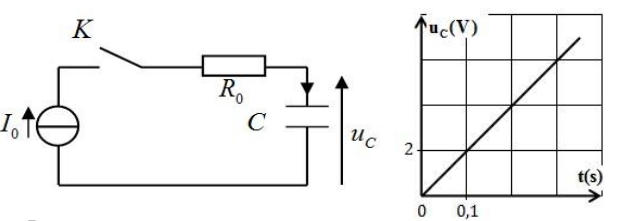
\includegraphics[width=0.6\textwidth]{./img/ex_02.png}
		%\captiocc{}
	\end{center}




\end{Box2}
\begin{Box2}{Exercice 3 : Réponse d’un dipôle RC à un échelon de tension }

	\begin{wrapfigure}[5]{r}{0.3\textwidth}
		\begin{center}
			\vspace{-0.6cm}
			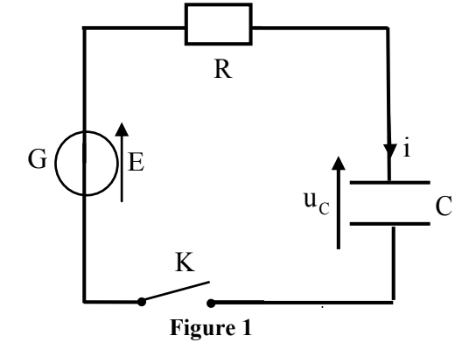
\includegraphics[width=0.26\textwidth]{./img/Ex33_c00.png}
			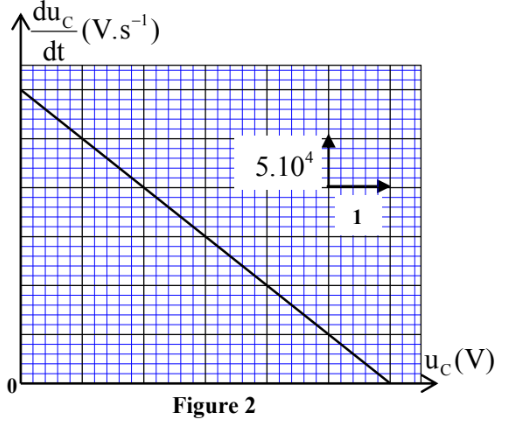
\includegraphics[width=0.3\textwidth]{./img/Ex33_c1.png}
		\end{center}
	\end{wrapfigure}



	On réalise le montage représenté sur le schéma de la figure 1. Ce montage comporte :
	\begin{itemize}
		\item un générateur de tension \( G \) de force électromotrice \( E \) ;
		\item un conducteur ohmique de résistance \( R = 2 \, \text{k}\Omega \) ;
		\item un condensateur de capacité \( C \) initialement déchargé ;
		\item un interrupteur \( K \).
	\end{itemize}

	À l’instant \( t = 0 \), on ferme \( K \). On note \( u_C \) la tension aux bornes \\du condensateur. La courbe de la figure 2 représente les variations \\de \( \frac{du_C}{dt} \) en fonction de \( u_C \).
	\begin{enumerate}
		\item Établir l’équation différentielle vérifiée par \( u_C \).
		\item Déterminer la valeur de \( E \) et vérifier que \( C = 10 \, \text{nF} \).
		\item On définit le rendement énergétique de la charge du condensateur par
		      $
			      \rho = \frac{E_e}{E_g}$
		      avec \( E_e \) l’énergie emmagasinée par le condensateur jusqu’au régime permanent et \( E_g = \frac{1}{2}C \cdot E^2 \) l’énergie fournie par le générateur \( G \). Déterminer la valeur de \( \rho \).
	\end{enumerate}


\end{Box2}

%%_________________________Exercice ! 3:"_________________________Exercice
\begin{Box2}{Exercice 4 : }

	\begin{wrapfigure}{r}{0.26\textwidth}
		\begin{center}
			\vspace{-0.8cm}
			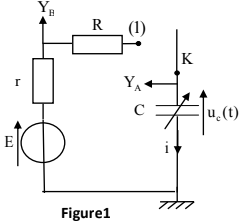
\includegraphics[width=0.26\textwidth]{./img/ex04_1.png}
			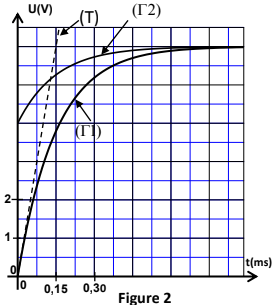
\includegraphics[width=0.26\textwidth]{./img/ex04_2.png}
			\caption{}
		\end{center}
	\end{wrapfigure}




	L’objectif de cet exercice est d’étudier la réponse d’un dipôle RC  à un échelon de tension .On réalise le circuit électrique schématisé sur la figure 1.Ce circuit comporte :
	\\Un générateur de f.e.m. E et de résistance
	interne négligeable ;
	\\- Deux conducteurs ohmiques de résistance r
	et $R=20\Omega$;
	\\- Un condensateur de capacité C réglable,
	initialement déchargé ;
	\\- Un interrupteur K .

	On fixe la capacité du condensateur sur la valeur $C_0$. A un instant de date $t=0$ , on place l’interrupteur
	K en position (1) .Un système d’acquisition informatisé permet de tracer les courbes $(\Gamma 1)$ et$(\Gamma 2)$ de la
	figure 2 représentant les tensions obtenues en utilisant les voies $Y_A$ et $Y_B$
	(fig.1) .La droite (T) représente la tangente à la courbe $(\Gamma 1)$ à t=0.

	\textbf{1. }Identifier parmi les courbes $(\Gamma 1)$ et $(\Gamma 2)$ celle qui représente la tension $u_C(t)$.

	\textbf{2. }Etablir l’équation différentielle vérifiée par la tension $u_C(t)$.

	\textbf{3. }Montrer que l’expression de l’intensité du courant juste après avoir placé l’interrupteur en position (1) est : $i_0 = \frac{E}{R+r}$

	\textbf{4. }A l’aide des deux courbes : Déterminer la valeur de r et Montrer que $C_0 = 5\mu.F$

\end{Box2}

%%_________________________Exercice 4 : _________________________Exercice
%\begin{Box2}{Exercice 4 :corde élastique }
%4
%\end{Box2}
%%\vspace{2cm}
%\begin{center}
%\Large{ \em{Exercices Supplémentaires}}
%\end{center}


%\vspace{-0.7cm}
%%%_________________________Exercice 5 : _________________________Exercice
%\begin{Box2}{Exercice 5 :Les ondes sonores }

%\end{Box2}
%%%_________________________Exercice 6 : _________________________Exercice
%\begin{Box2}{Exercice 6 : échographie}

%\end{Box2}

\end{document}
